\chapter{نحوه‌ی استقرار مدل و تکنولوژی‌های استفاده‌شده}

در این بخش ابتدا تکنولوژی‌ها و چارچوب\LTRfootnote{Framework}‌های اصلی دخیل در توسعه این دستگاه را به طور دقیق مورد بررسی قرار می‌دهیم و در قسمت بعد به طریقه‌ی استقرار\LTRfootnote{Deployment} مدل یادگیری ماشین سیستم پیاده‌شده اشاره می‌کنیم. شایان ذکر است که مدل یادگیری ماشین به صورت یک سرویس مجزا به کارگزار\LTRfootnote{Server} 
جمع‌آوری اطلاعات لرزش گره‌ها که در یک پروژه‌ی مجزا در راستای پروژه‌ی کنونی توسعه یافته است، اضافه شده است.

\section{‌‌زبان برنامه‌نویسی}
برای انتخاب زبان برنامه‌نویسی مناسب برای توسعه مدل یادگیری ماشین شرح‌داده شده، باید معیارهای متفاوتی را در نظر گرفت. برای این منظور زبان پایتون\LTRfootnote{\href{https://docs.python.org/3/}{Python}} را برگزیدیم. مواردی همچون داشتن چارچوب‌ها و کتابخانه‌های قدرتمند یادگیری ماشین، توسعه‌ی آسان و سریع و محبوبیت بالا از دلایل اصلی انتخاب پایتون به عنوان زبان اصلی برای توسعه‌ی سرویس یادگیری ماشین می‌باشد. همچنین شایان ذکر است که چون کارگزار اصلی جمع‌آوری اطلاعات لرزش به زبان پایتون نوشته شده است، استفاده از این زبان برای توسعه مدل یادگیری ماشین، باعث بهبود توسعه‌پذیری نیز می‌گردد. 

\subsection{زبان برنامه‌نویسی پایتون}
یک زبان برنامه‌نویسی عمومی و سطح بالا است که فلسفه طراحی آن بر روی خوانایی کد تأکید دارد. نحو\LTRfootnote{Syntax} پایتون به برنامه‌نویسان امکان می‌دهد تا مفاهیم را با تعداد کمتری خط کد نسبت به زبان‌هایی مانند سی\LTRfootnote{C Programming Language} بیان کنند و این زبان ساختارهایی را فراهم می‌کند که برنامه‌های واضح و قابل فهم را در هر دو مقیاس کوچک و بزرگ فراهم می‌سازد\cite{van2007python}. یکی از مشخصه‌های مهم پایتون این است که از چندین الگو\LTRfootnote{Paradigm}ی برنامه‌نویسی، از جمله شیءگرا\LTRfootnote{Object Oriented Programming (OOP)} و تابعی یا روش‌های رویه‌ای، پشتیبانی می‌کند. پایتون سیستم نوع پویا و مدیریت خودکار حافظه را پشتیبانی می‌کند و کتابخانه‌های استاندارد و جانبی بزرگ و جامع دارد. مفسرهای پایتون برای بسیاری از سیستم‌عامل‌ها در دسترس هستند\cite{srinath2017python}. از جمله مهم‌ترین ویژگی‌های پایتون می‌توان به موارد زیر اشاره کرد.

\begin{itemize}

\item \textbf{سادگی}: پایتون یک زبان برنامه‌نویسی بسیار سطح بالا است که منابع زیادی برای یادگیری آن وجود دارد. پایتون از ابزارهای شخص ثالث متنوعی پشتیبانی می‌کند که استفاده از آن را بسیار آسانتر می‌کند و کاربران را ترغیب می‌کند تا ادامه دهند\cite{srinath2017python, sharma2020python}.

\item \textbf{متن‌باز بودن\LTRfootnote{Open Source}}: اگرچه تمام حقوق این زبان برنامه‌نویسی متعلق به سازمان پایتون است، اما درحال‌ حاضر به عنوان یک نرم‌افزار متن‌باز وجود دارد و هیچ محدودیتی در استفاده، تغییر و توزیع آن وجود ندارد. شما می‌توانید به آزادی از پایتون استفاده کنید و آن را برای استفاده شخصی و یا تجاری توزیع کنید. نه تنها می‌توانید نرم‌افزاری که با آن نوشته شده است را استفاده و توزیع کنید، بلکه حتی می‌توانید تغییراتی در خود کد منبع پایتون اعمال کنید. همچنین شایان ذکر است که پایتون یک جامعه بزرگ و پویا دارد که در هر نسخه آن را بهبود می‌بخشد\cite{srinath2017python, sharma2020python}.

\item \textbf{کتابخانه‌ها وچارچوب‌ها}: پایتون دارای یک سری کتابخانه‌های استاندارد و چارچوب‌های متنوع است که کار برنامه‌نویسان را بشدت راحت می‌کند، زیرا نیازی نیست تمام کدنویسی را خود برنامه‌نویس انجام دهد. کتابخانه‌های استاندارد در پایتون به خوبی تست شده‌اند و توسط هزاران نفر استفاده می‌شوند. بنابراین، می‌توان اطمینان داشت که استفاده از این کتابخانه‌ها توانایی ایجاد خرابی در برنامه‌های شما را ندارند\cite{srinath2017python, sharma2020python}.

\end{itemize}

حال به بررسی معایب پایتون می‌پردازیم. نکته‌ی قابل توجه در این قسمت این است که اگر معایب نام‌برده شده تاثیر زیادی در کیفیت خدمت ارائه‌شده به کاربر بگذارند، استفاده از پایتون اصلا توصیه نمی‌شود و باید به دنبال جایگزینی مناسب گشت. از جمله کاستی‌های پایتون عبارت‌اند از:

\begin{itemize}

\item \textbf{کندی}: به عنوان یک زبان با نوع پویا، پایتون به دلیل انعطاف‌پذیری بالا، کند عمل می‌کند، زیرا ماشین باید بسیاری از مراجعات را انجام دهد تا از تعریف چیزی مطمئن شود و این باعث کاهش عملکرد پایتون می‌شود\cite{srinath2017python, sharma2020python}.

\item \textbf{دشواری فرایند نگهداری\LTRfootnote{Maintaining}}: به دلیل اینکه پایتون یک زبان با نوع پویا است، یک چیز ممکن است به راحتی به معنای متفاوتی در تک‌نمایی متفاوت تفسیر شود. با افزایش اندازه و پیچیدگی یک برنامه پایتون، نگهداری آن ممکن است دشوار شود. با کمک تست‌های واحد\LTRfootnote{Unit Tests} می‌توان تا حدی این از وقوع این مشکل جلوگیری کرد\cite{srinath2017python, sharma2020python}.

\end{itemize}



\section{چارچوب‌ها}



\section{استقرار مدل یادگیری ماشین}
پس از پیاده‌سازی مدل یادگیری ماشین، نیاز است که به طریقی سیستم را در دسترس همگان قرار داد تا بتوان از مزایای آن استفاده کرد. شرکت‌های ارائه‌دهنده‌ی خدمات ابری\LTRfootnote{Cloud Services Providers} یا به اختصار \lr{CPS}، گزینه‌ی مناسبی برای این نیاز می‌باشد. برای این منظور، ما این پروژه را پس از پیاده‌سازی، توسط سرویس زیرساخت به عنوان خدمت\LTRfootnote{Infrastructure as a Service (IaaS)} مستقر کردیم.

\subsection{زیرساخت به عنوان خدمت}
در این مدل، سرویس‌دهنده ابر یا \lr{CPS} مجموعه‌ای از منابع محاسباتی مجازی شده را در ابر فراهم می‌کند (مانند پهنای باند شبکه، ظرفیت ذخیره‌سازی، حافظه، قدرت پردازش). مسئولیت مشتری در این حالت این است که سیستم‌عامل و برنامه‌های نرم‌افزاری را روی این منابع مجازی اجرا و نگهداری کند. زیرساخت به عنوان خدمت یا \lr{IaaS} از فناوری مجازی‌سازی استفاده می‌کند تا منابع فیزیکی را به منابع منطقی تبدیل کند که مشتریان می‌توانند به صورت پویا از آنها استفاده کنند و آنها را هنگام نیاز ایجاد و آزاد کنند\cite{youssef2012exploring}. در \cref{fig:different_cloud_services} نمای کلی سرویس‌های مختلف موجود در یک سیستم ابری را مشاهده می‌کنیم. همانطور که مشخص است در \lr{IaaS}، کاربر بیشترین کنترل را بر روی منابع در اختیار گذاشته‌شده دارد\cite{serrano2015infrastructure}.



\begin{figure}[!h]
\centerline{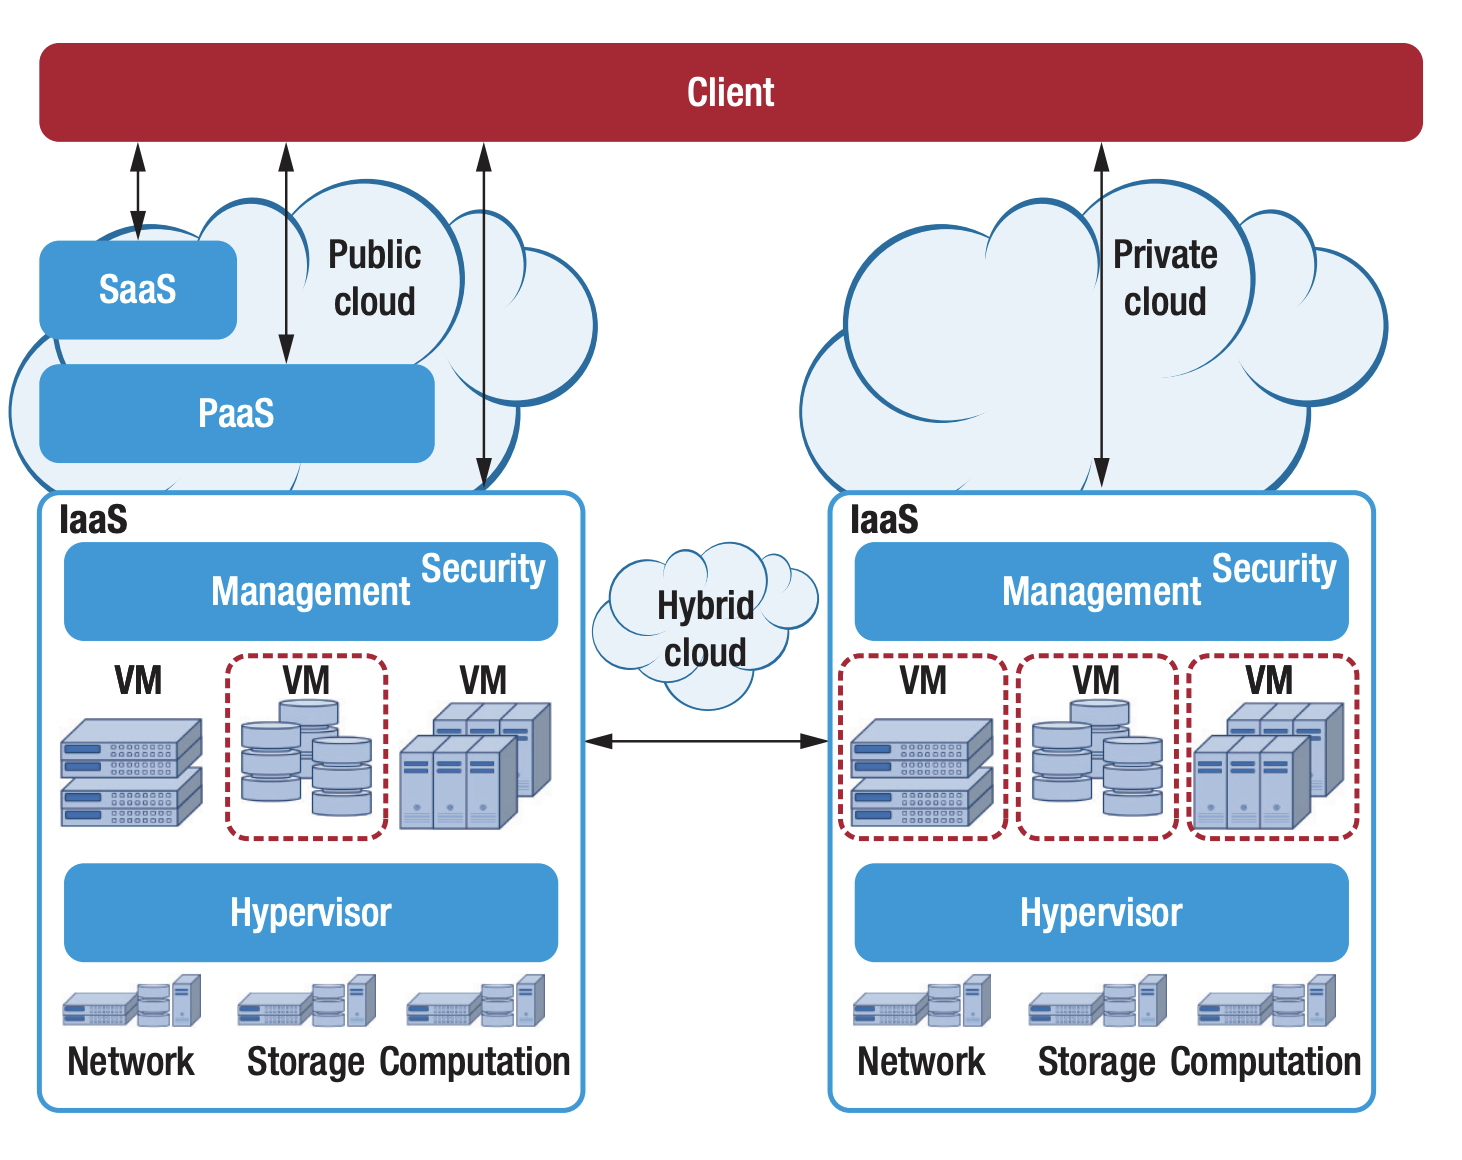
\includegraphics[width=\textwidth]{different_cloud_services.png}}
\caption{انواع سرویس‌های ارائه‌شده توسط شرکت‌های خدمات ابری}
\label{fig:different_cloud_services}
\end{figure}


\subsection{انواع روش‌های استقرار}
 روش‌های مختلفی برای استقرار و استفاده از مدل‌های یادگیری هوش مصنوعی مورد استفاده قرار می‌گیرند که از بین اینها چهار روش نشان داده‌ شده در \cref{fig:ml_model_deployments} مرسوم‌تر هستند\cite{kaggleMLdeployments}:

\begin{figure}[!h]
\centerline{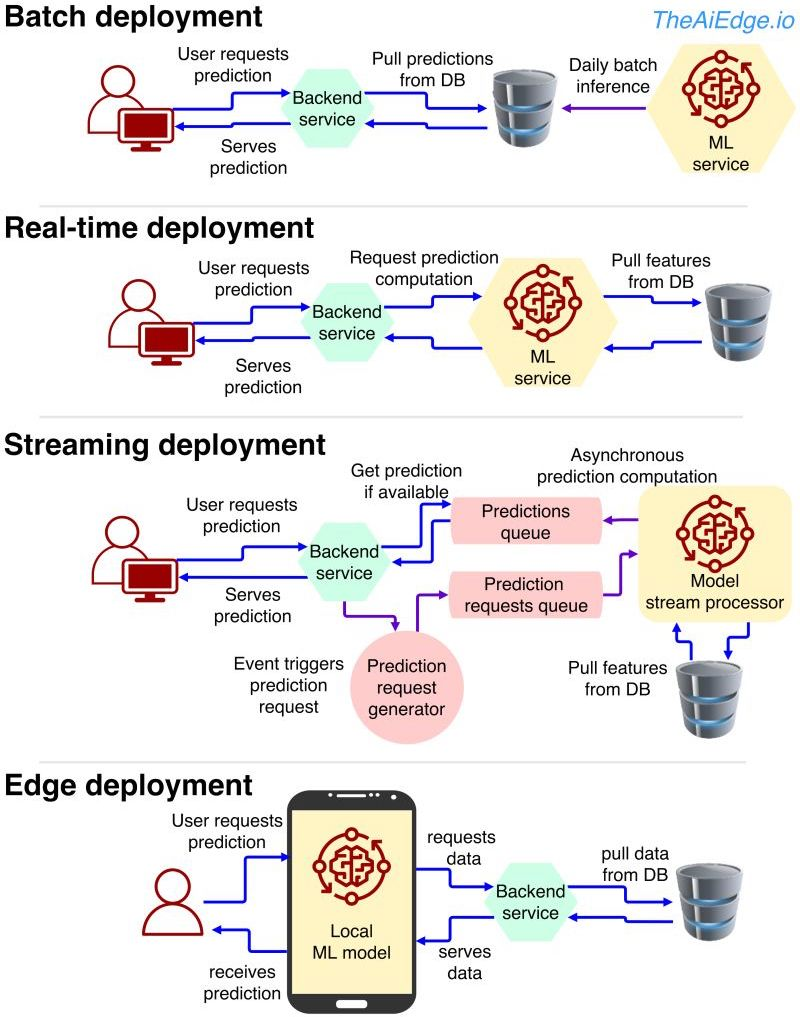
\includegraphics[width=.5\textwidth]{ml_model_deployments.png}}
\caption{انواع روش‌های استقرار مدل‌های یادگیری ماشین}
\label{fig:ml_model_deployments}
\end{figure}

\begin{itemize}

\item \textbf{پیاده‌سازی دسته‌ای\LTRfootnote{Batch Deployment}}: پیش‌بینی‌ها به فاصله‌های زمانی مشخص محاسبه می‌شوند و پیش‌بینی‌های حاصل در پایگاه داده ذخیره می‌شوند و به راحتی می‌توان آنها را در صورت نیاز بازیابی کرد. با این حال، نمی‌توان از داده‌های بروزتر استفاده کرد و پیش‌بینی‌ها می‌توانند به سرعت منسوخ شوند\cite{singh2021deploy, pacheco2018towards}.

\item \textbf{پیاده‌سازی بی‌درنگ\LTRfootnote{Real-Time Deployment}}: در این نوع از استقرار، درخواست کاربر برای گرفتن جدید‌ترین پیش‌بینی‌ها به عنوان یک راه‌انداز\LTRfootnote{Trigger} توسط رابط برنامه‌نویسی\LTRfootnote{Application Programming Interface (API)} اچ‌تی‌تی‌پی\LTRfootnote{Hypertext Transfer Protocol (HTTP)} به کارگزار ارسال می‌شود. سپس سرویس یادگیری ماشین که به عنوان افزونه‌ای در سمت کارگزار توسعه یافته است، شروع به کار می‌کند و جدیدترین نتایج پیش‌بینی را تولید و ذخیره می‌کند و به سمت کاربر به عنوان نتیجه ارسال می‌کند. مشکل اصلی این روش قرارگیری مدل یادگیری ماشین، کند بودن روند یادگیری و پیش‌بینی است که منجر به منتظر ماندن کاربر می‌گردد. می‌توان با بهره‌گیری از فرآیند\LTRfootnote{Process}‌های چندریسمانی\LTRfootnote{Multi-Threaded} برای دریافت درخواست‌های کاربر و انجام مرحله‌ی یادگیری و پیش‌بینی مدل، تا حد زیادی این مشکل را برطرف کرد\cite{singh2021deploy, pacheco2018towards}.

\item \textbf{پیاده‌سازی جریانی\LTRfootnote{Streaming Deployment}}: این امکان را می‌دهد تا فرآیند ناهمزمان‌\LTRfootnote{Asynchronous}تری ایجاد شود. یک رویداد می‌تواند شروع فرآیند استنتاج را فراهم کند. این فرآیند در صف یک واسط پیام\LTRfootnote{Message Broker} مانند کافکا\LTRfootnote{Apache Kafka} قرار داده می‌شود و مدل یادگیری ماشینی در هنگام آماده شدن برای انجام درخواست، آن را انجام می‌دهد. این کار به سرویس پشتیبانی فرصت می‌دهد و با فرآیند صف بهینه، قدرت محاسباتی بسیاری را صرفه‌جویی می‌کند. پیش‌بینی‌های حاصل شده نیز در صف قرار گرفته و در صورت نیاز توسط سرویس‌های پشتیبانی مصرف می‌شوند. از مزیت‌های این روش نسبت به روش بی‌درنگ، می‌توان به کم‌شدن تاخیر پاسخ‌دهی به کاربران اشاره کرد\cite{singh2021deploy, pacheco2018towards}.

\item \textbf{پیاده‌سازی لبه‌ای\LTRfootnote{Edge Deployment}}: در این روش استقرار، مدل مستقیماً بر روی کلاینت نصب می‌شود، مانند مرورگر وب، یک تلفن همراه یا محصولات اینترنت اشیاء. این کار باعث رسیدن به سریع‌ترین استنتاج می‌شود، اما معمولاً مدل‌ها باید به اندازه کافی کوچک باشند تا بتوانند در سخت‌افزارهای کوچکتر نصب شوند\cite{kaggleMLdeployments}.

\end{itemize}

بدلیل اینکه گره‌های موجود در شبکه‌ی اشیاء دارای توان پردازشی محدود هستند و اینکه ماهیت مدل هوش‌ مصنوعی مربوط به حوزه‌ی کاری پیش‌بینی عمر دستگاه‌ها بدین‌گونه است که حتما باید از داده‌های مربوط به همه‌ی گره‌های موجود استفاده کرد، با توجه به گزینه‌های مطرح‌شده برای استقرار مدل هوش مصنوعی توسعه‌داده شده و همچنین مزایا و معایب هر کدام، از روش استقرار بی‌درنگ برای ارائه و بکارگیری مدل هوش مصنوعی در این پروژه استفاده شده است. به طور دقیقتر، مدل هوش مصنوعی به عنوان یک سرویس اضافی برای کارگزار اصلی توسعه‌ داده‌شده در پروژه‌ی مرتبط 
به این پروژه تعبیه شده است. 

